%!TEX root = ../Thesis.tex

% 4. Analysis
% Your analysis, along with your discussion, will form the high light of your thesis. In the IMRaD format, this section is titled “Results”. This is where you report your findings and present them in a systematic manner. The expectations of the reader have been built up through the other chapters, make sure you fulfil these expectations.

% To analyse means to distinguish between different types of phenomena – similar from different. Importantly, by distinguishing between different phenomena, your theory is put to work. Precisely how your analysis should appear, however, is a methodological question. Finding out how best to organise and present your findings may take some time. A good place to look for examples and inspiration is repositories for master’s theses.

% If you are analysing human actions, you may want to engage the reader’s emotions. In this case, it will be important to choose analytical categories that correlate to your chosen theory. Engaging emotions is not the main point, but a way to elucidate the phenomenon so that the reader understands it in a new and better way.

% Note: Not all theses include a separate chapter for analysis.

\chapter{Analysis}

\section{Pump control}
To check the declared functionality of pump control I have made a test setup where motor's thermoresistors can be replaced with matched potentiometers. In this manner, I could fully control the temperatures sensed in the very beginning of the system and what is important without any modifications to the final version of the software.
\newline
\newline
I have captured 10 state transitions to demonstrate the whole spectrum of changes as follows.
\begin{description}
    \item[Temperature set to 30\textdegree C and varying accelerator displacement] \hfill \\ Expected behaviour of pumps output would be to raise proportionally from 2,5V for pedal in initial position up to 5V whenever it is pressed up to its limit.
    \item[Temperature set to 35\textdegree C and varying accelerator displacement] \hfill \\ Same behaviour as explained above.
    \item[Temperature set to 40\textdegree C and varying accelerator displacement] \hfill \\ Same behaviour as explained above.
    \item[Temperature set to 45\textdegree C and varying accelerator displacement] \hfill \\ Initial pump output should equal to $2,5V + 2,5V*25\% = 3,125V$ and saturate on pedal displacement of $75\% $.
    \item[Temperature set to 50\textdegree C and varying accelerator displacement] \hfill \\ Initial pump output should equal to $2,5V + 2,5V*50\% = 3,75V$ and saturate on pedal displacement of $50\% $.
    \item[Temperature set to 55\textdegree C and varying accelerator displacement] \hfill \\ Initial pump output should equal to $2,5V + 2,5V*75\% = 4,375V$ and saturate on pedal displacement of $25\% $.
    \item[Temperature set to 60\textdegree C and varying accelerator displacement] \hfill \\ Initial pump output should equal to maximum value of $5V$ and pedal displacement should not affect this value.
    \item[Temperature set to 65\textdegree C and varying accelerator displacement] \hfill \\ Same behaviour as explained above.
    \item[Temperature set to 70\textdegree C and varying accelerator displacement] \hfill \\ Same behaviour as explained above.
\end{description}
\begin{description}
    \item[Varying temperature from 30 to 70 degrees and no accelerator displacement] \hfill \\ Pump output should vary from $2,5V$ and $5V$ being in direct proportion to temperature changes from 40 to 60 degrees.
\end{description}

Taking for instance measurement for temperature set $50\deg C$ and pressing acceleration pedal. I have had captured severely noisy signal from accelerator sensor and temperature sensor emulator then prepossessed them in a similar manner as it is done inside the system\footnote{average of 50 consecutive samples}. The sensors output, as well as pumps controlling signal, has been shown in the figure \ref{pump_50}.

\begin{figure}[h]
    \centering
    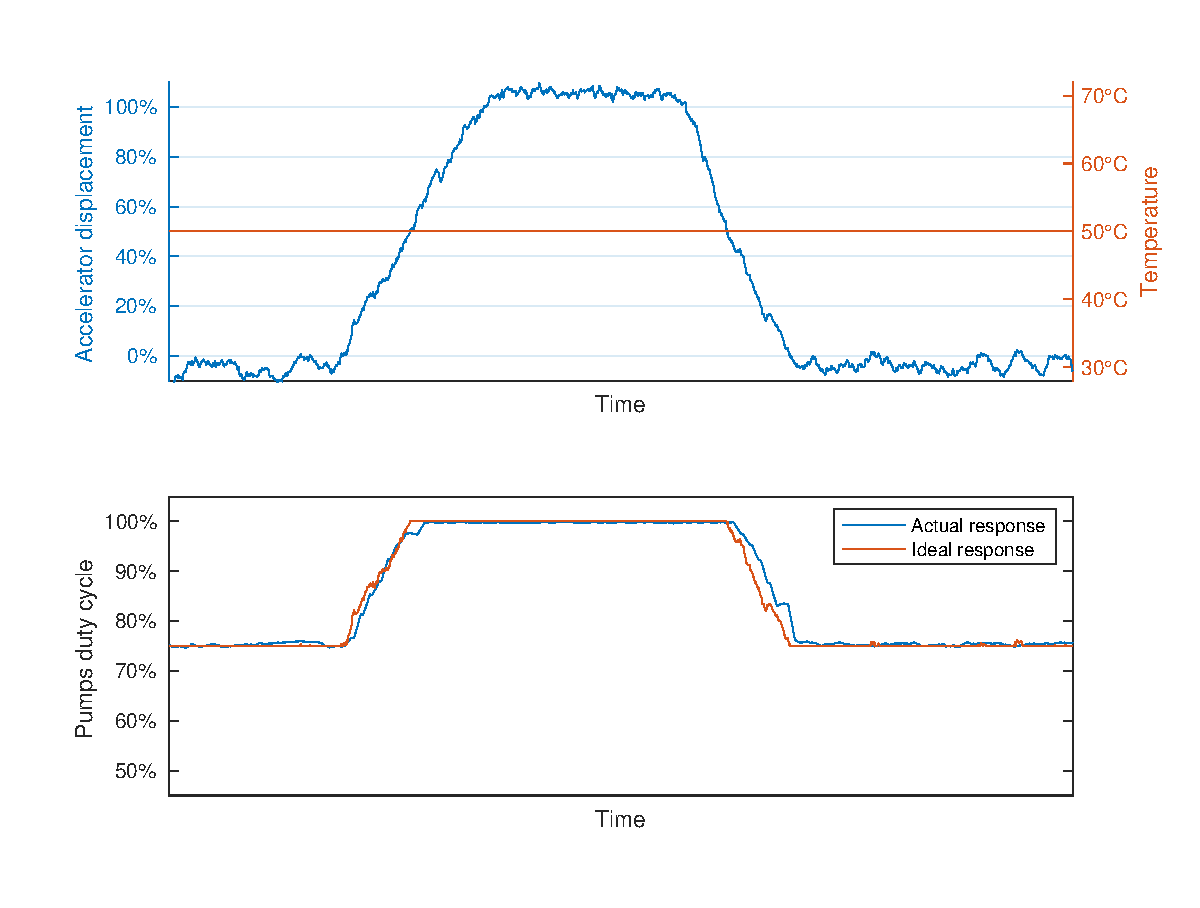
\includegraphics[height=5.8cm]{figures/pump_50.eps}
    \caption[Temperature set to 50\textdegree C and varying accelerator displacement]{Comparison of actual pump control signal to idealised one based on the same input data}
    \label{pump_50}
\end{figure}

In the same figure, I have plot theoretical output based on an idealised mathematical model. As one can notice control output closely follows the desired patch. The only visible difference is due to the fact that in my system the control signal is intentionally delayed.
The pumps control signal is updated only once per 100 milliseconds since temperature change is rather a slow process in this way we can avoid harmful (for pumps) high-frequency oscillations and save computation power. In this way, we obtain a simple control system with memory which is even more visible if we just plot input against output (accelerator/control signal) which has been done in \ref{pump_50_1}. In the graph, we can observe the hysteresis and steps upon control update as we could expect.


\begin{figure}[h]
    \centering
    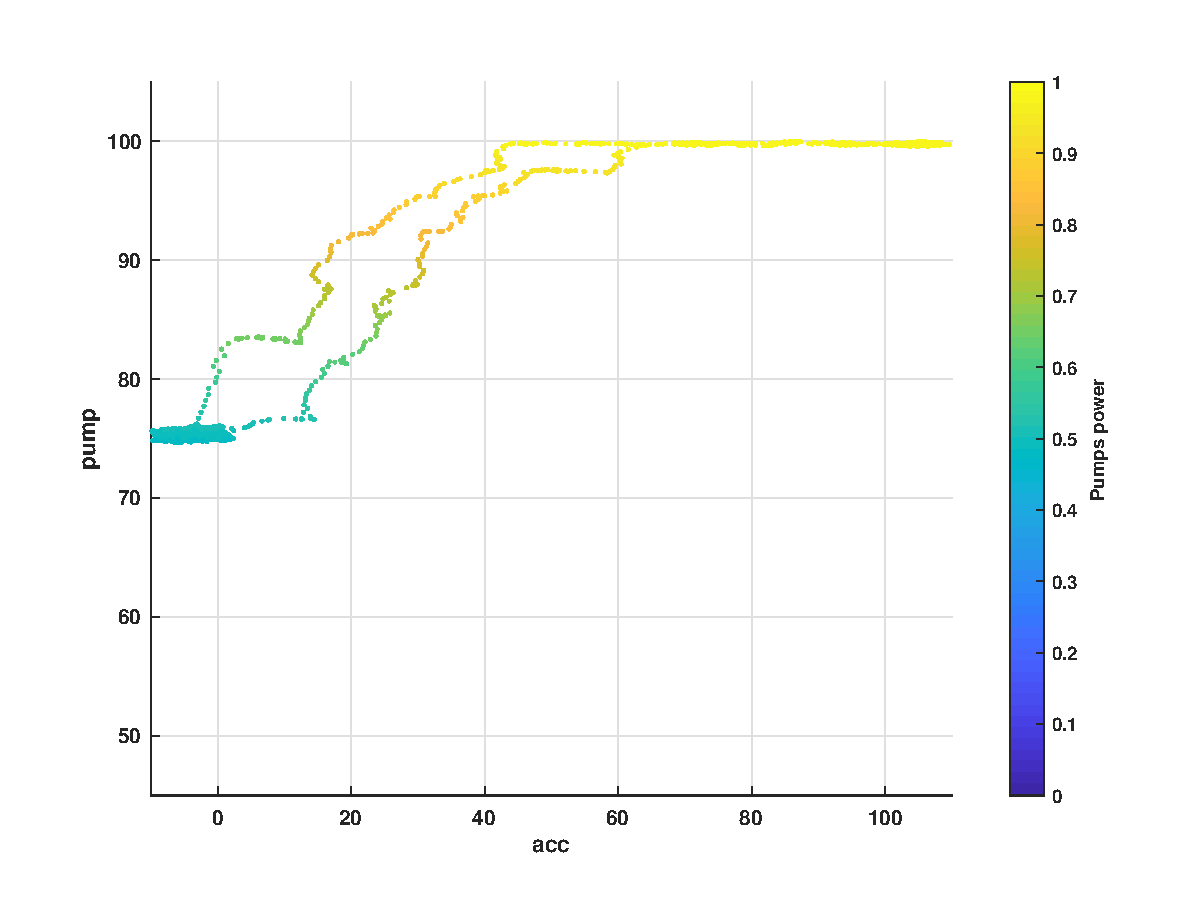
\includegraphics[height=5.8cm]{figures/pump_50_1.eps}
    \caption[Accelerator displacement against pump output]{Accelerator displacement against pump output (samples sorted based accelerator position)}
    \label{pump_50_1}
\end{figure}

I have repeated this process for all above-mentioned cases confirming that this sub-system works correctly. The figures for all the other cases can be found in appendix \ref{pumps_graphs}. To present all the results in the clear graphical way I have combined them into scatter chart plotting the accelerator against temperature values and colour mapping them by measured output \ref{Raw_pump_sum}. To show the validity of data on the right you can see the same graph with the background coloured based on a mathematical model.

\begin{figure}[h]
    \centering
        \subbottom[Measured controlling signal]{
            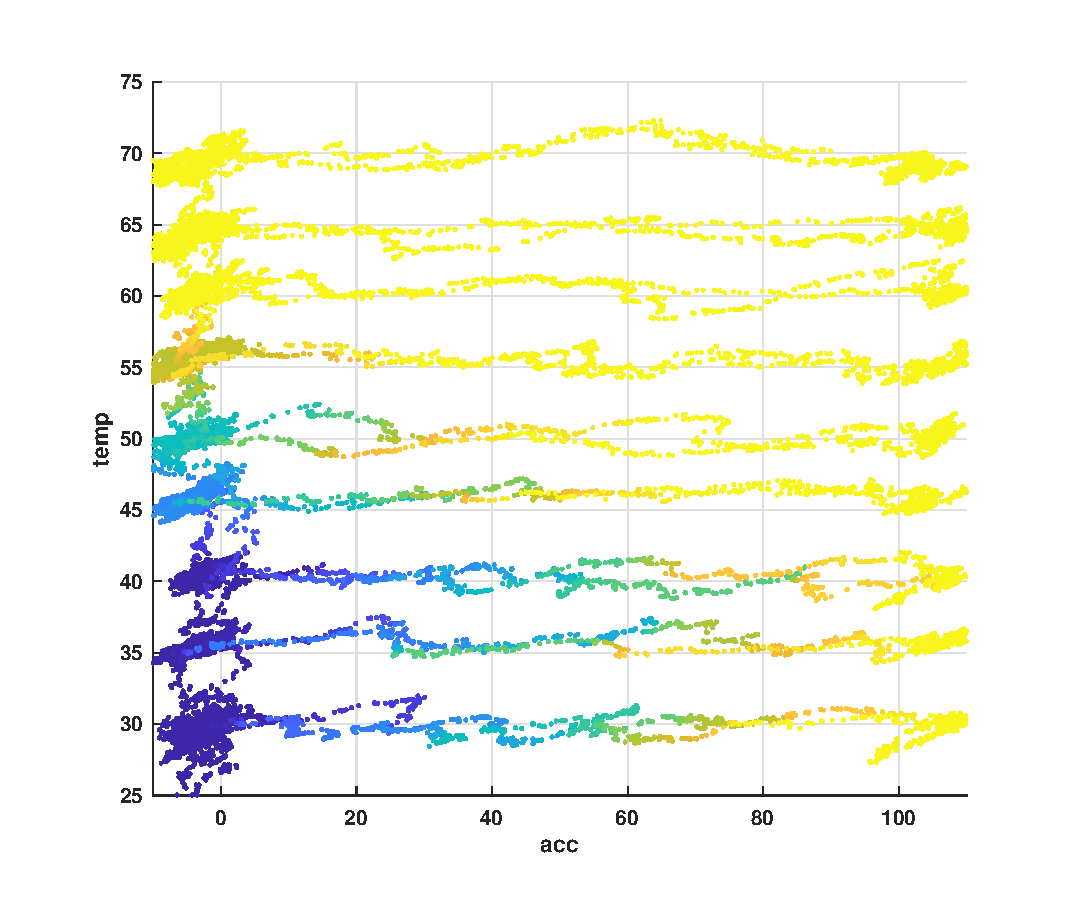
\includegraphics[height=5.8cm]{figures/Pumps_summary_raw.eps}
            \label{Raw_pump_sum}
        }
        ~
        \subbottom[With shading based on the model]{
            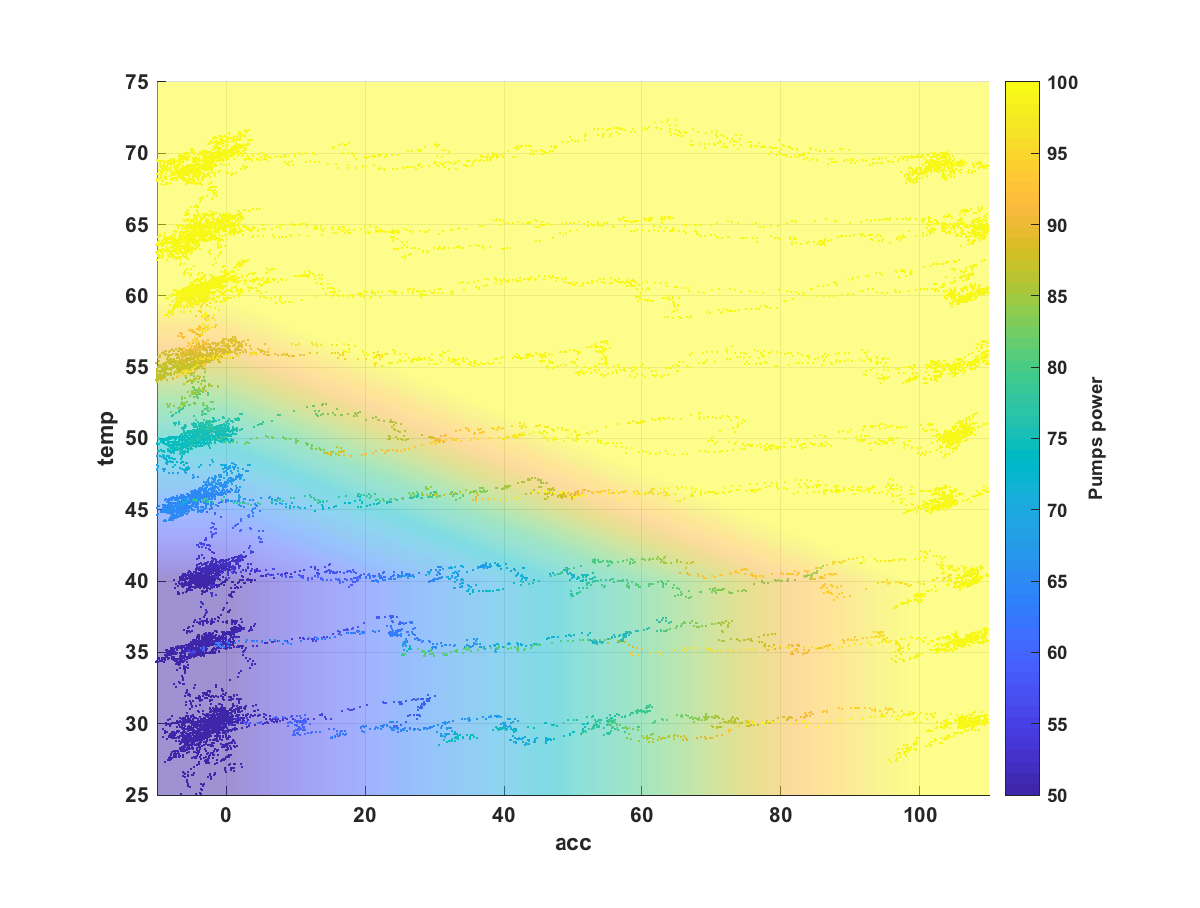
\includegraphics[height=5.8cm]{figures/Pumps_summary.eps}
            \label{Shaded_pump_sum}
        }
        \caption{Pumps control summary}
    \label{Pump_sum}
\end{figure}

\section{Regenerative Breaking}
Due to the fact that the car battery has not been finished, I have been required to make the measurements on setup powered by a laboratory amplifier. This greatly narrowed the spectrum in which I could check if the system operates correctly.

As the amplifier did not accept backward current and the car could not be driven I could not measure actual regenerative breaking. On the other hand limited current reduced dynamics of the setup and having the wheels freely spinning in the air became safely issue for high torque/speed.

To prove the validity of the programme I have measured the torque with accompanying speed for the acceleration pedal displacement from $0$ to $25\%$. As mentioned in the method section \ref{speed_mode} for first $15\%$  the control system has negative feedback loop effectively making the speed of the vehicle linearly proportional to the pedal displacement.
The pedal position has been changed by $1\%$ on each second as shown in \ref{torq_anal}. 

% \begin{wrapfigure}{!r}{0.5\textwidth}
%     \vspace{-20pt}
%     \begin{center}
%     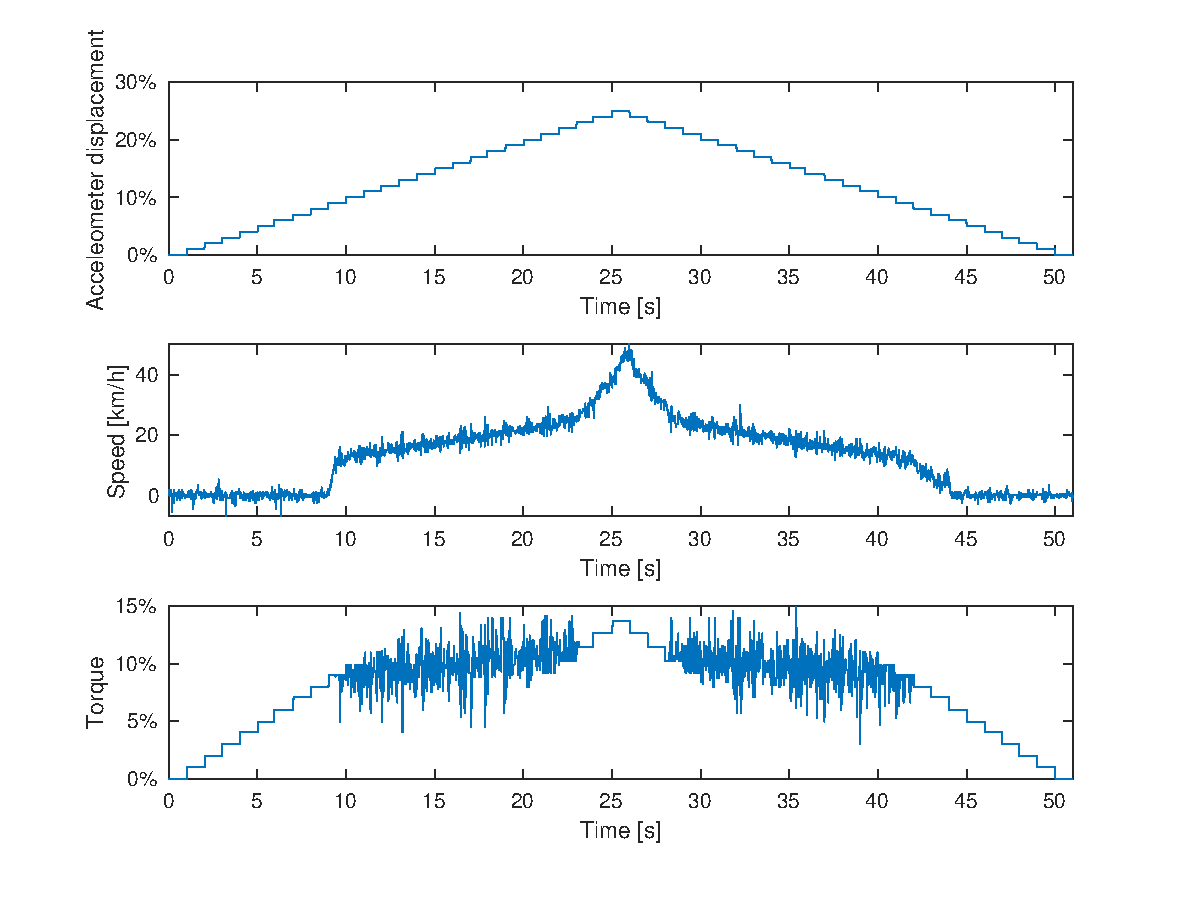
\includegraphics[width=0.48\textwidth]{figures/torq_anal}
%     \label{torq_anal}
%     \end{center}
%     \caption{Test signal for accelerator displacement}
%     \vspace{-20pt}
% \end{wrapfigure}

As expected torque output from the system was a reflection of pedal positions as long as the wheels did not spin and for speeds from $10-20 km/h$ we can observe linear dependency between pedal and speed. Then for the speeds above $20km/h$ there is simple torque control so the wheels (without load) starts to gain speed in exponential tempo.

To put in the bigger picture let me refer to the theoretical model (\ref{fig:regen_ideal}). In the figure \ref{torq_anal} I present the measured output using the idealised model as the background. 


\begin{figure}[h]
    \centering
        \subbottom[Test signal for accelerator displacement]{
            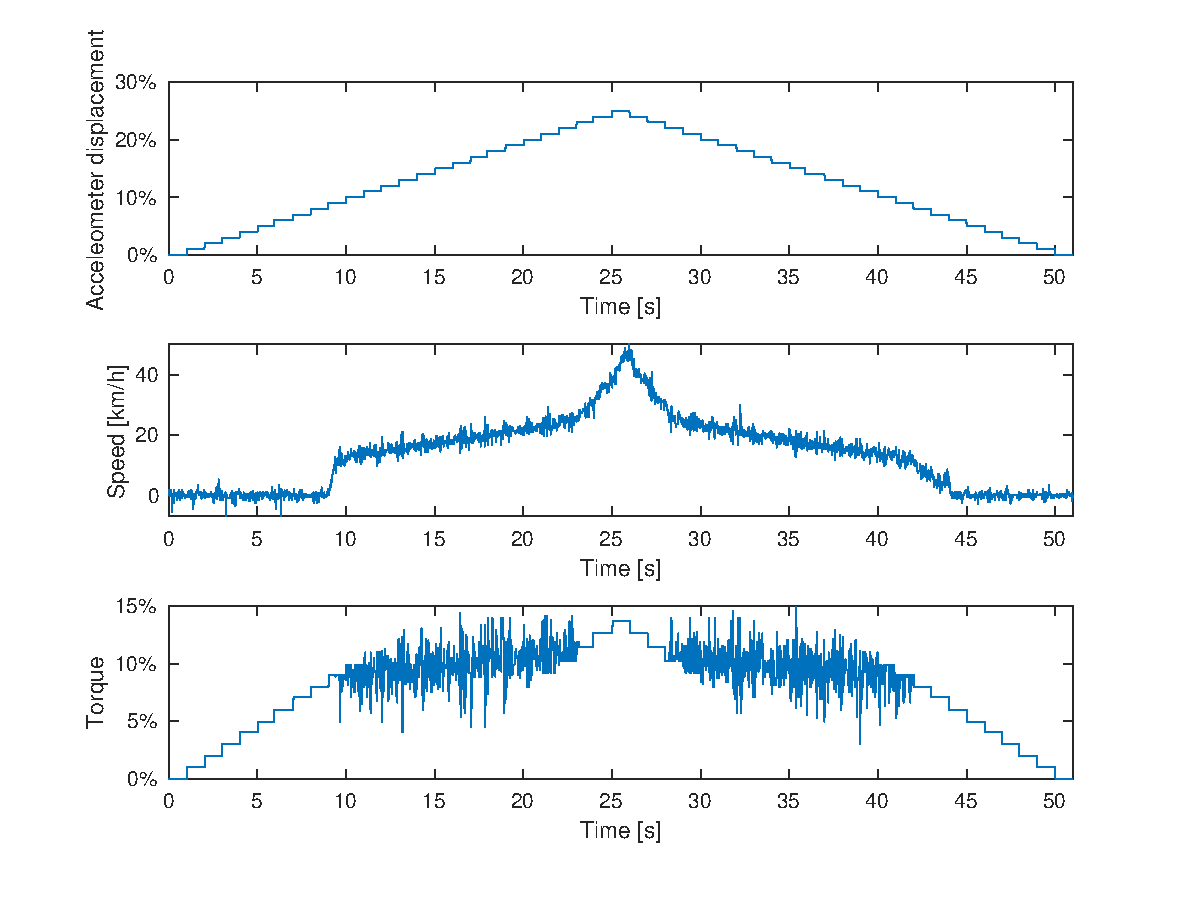
\includegraphics[width=0.46\textwidth]{figures/torq_anal}
            \label{torq_anal}
            %\caption{Test signal for accelerator displacement}
        }
        ~
        \subbottom[Measured correlation against idealised model]{
            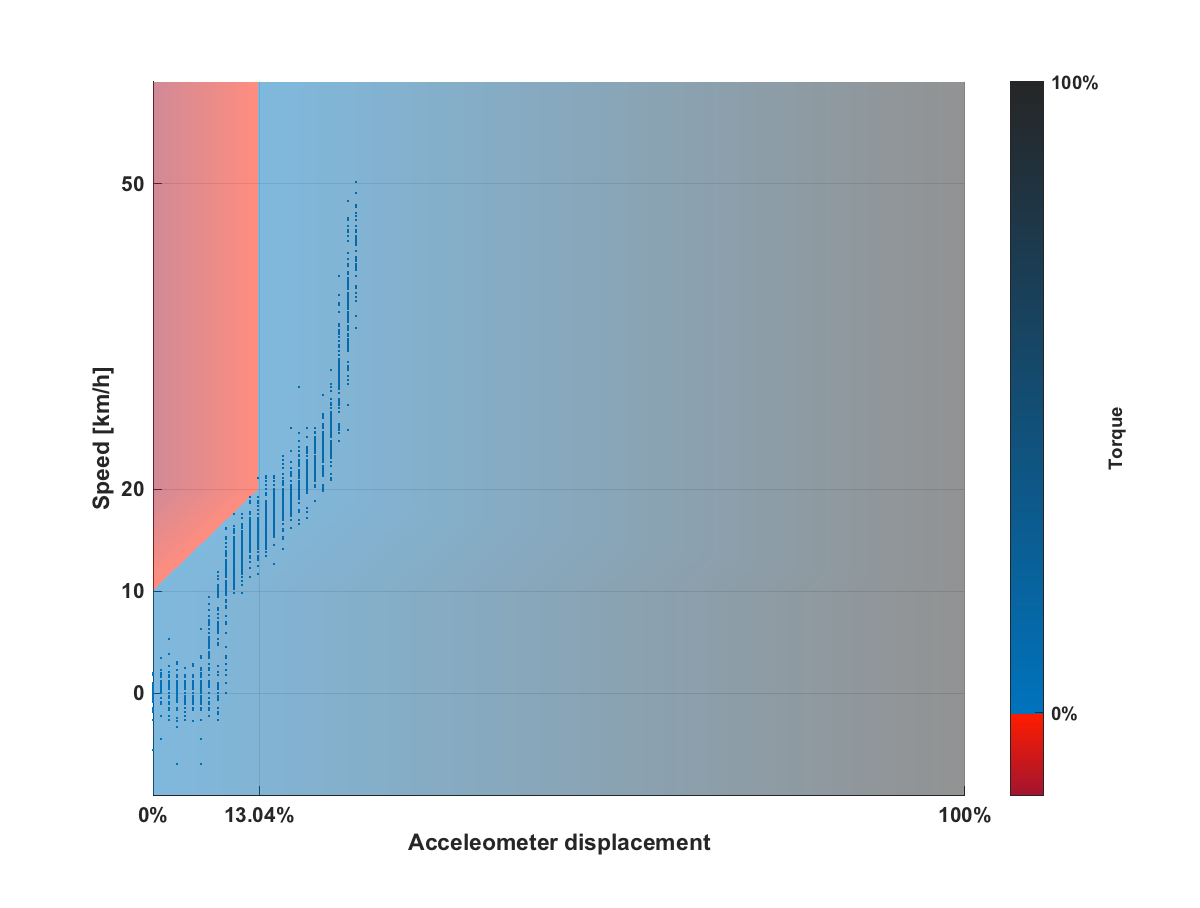
\includegraphics[width=0.46\textwidth]{figures/regen_anal.eps}
            %\caption{Measured correlation against idealised model}
            \label{regen_anal}
        }
        \caption{Torque control summary}
    \label{torq_ctl}
\end{figure}

% \begin{figure}[h]
%     \centering
%         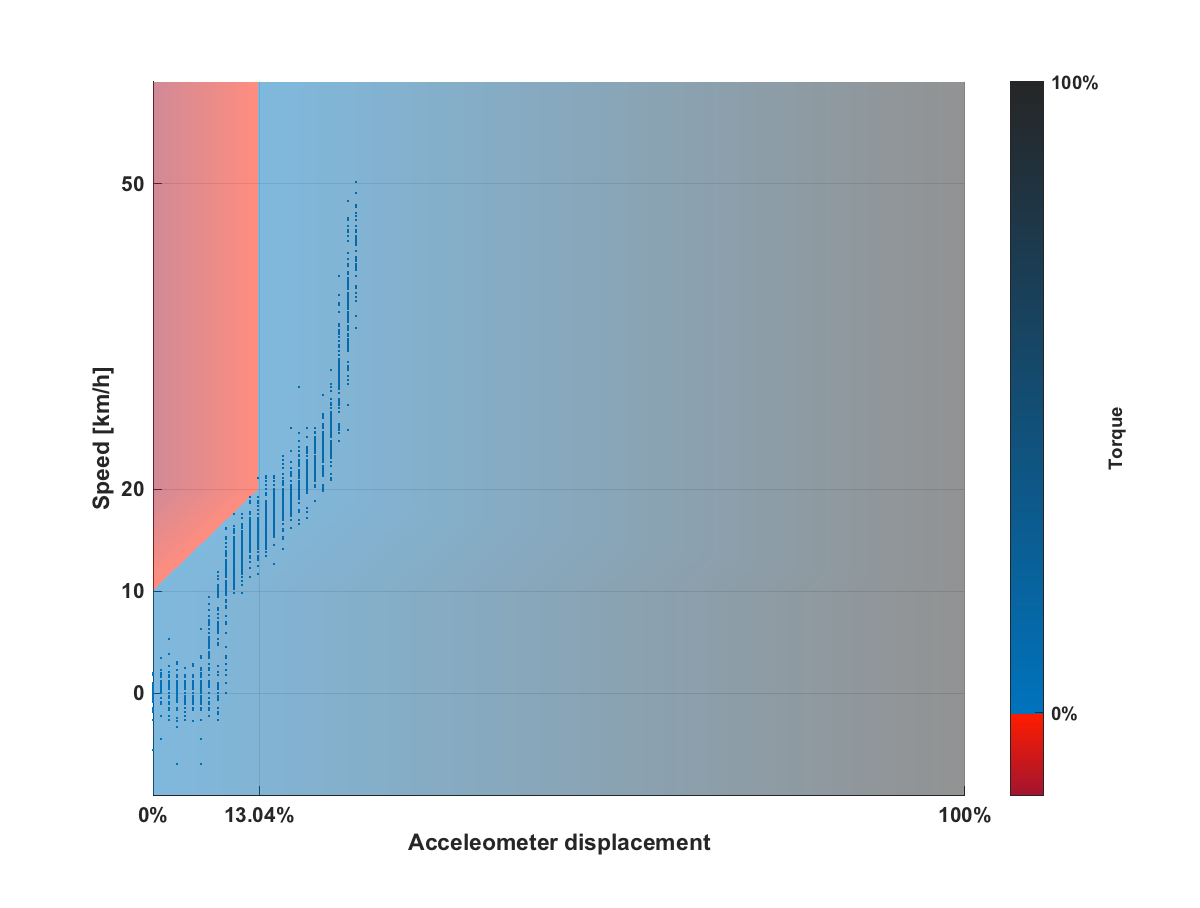
\includegraphics[height=5.8cm]{figures/regen_anal.eps}
%         \caption{Measured correlation against idealised model}
%         \label{regen_anal}
% \end{figure}

Beside above-mentioned dependencies, one can observe that there is the initial value of torque needed for a wheel to start spinning and around half a value torque to maintain its angular momentum. 

\section{Differential}
To confirm the validity of implemented model I have commit measurements where the steering wheel was rotated for each $~5\%$ displacement of acceleration pedal and where acceleration pedal was pressed fully for seemingly equally distributed 21 positions of the steering wheel in its full scale of operation. Detailed measurements results can be found in appendix \ref{diff_app}.

Meanwhile, the summarised version can be seen in figure \ref{diff_sum}.

\begin{figure}[h]
    \centering
        \subbottom[]{
            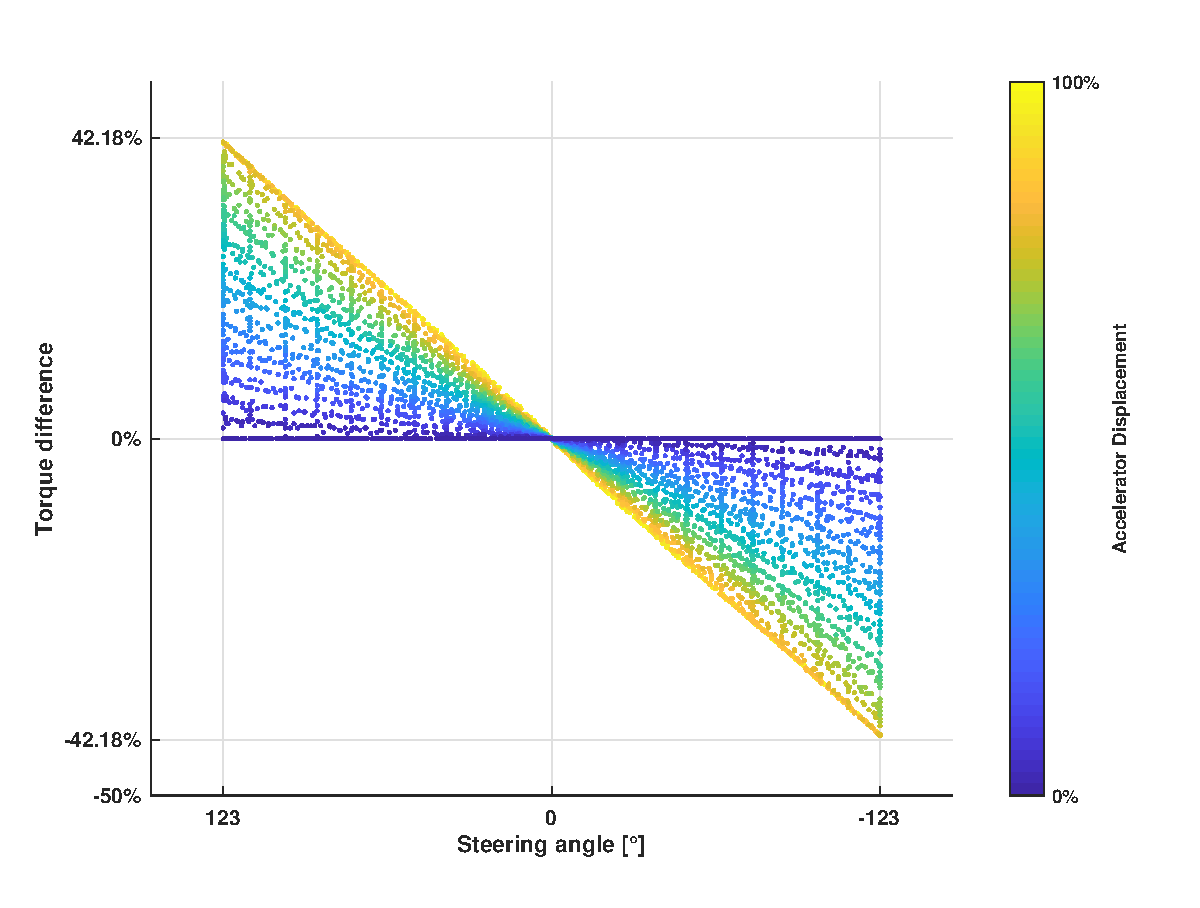
\includegraphics[width=0.46\textwidth]{figures/ste_torq.eps}
            \label{}
            %\caption{Test signal for accelerator displacement}
        }
        ~
        \subbottom[]{
            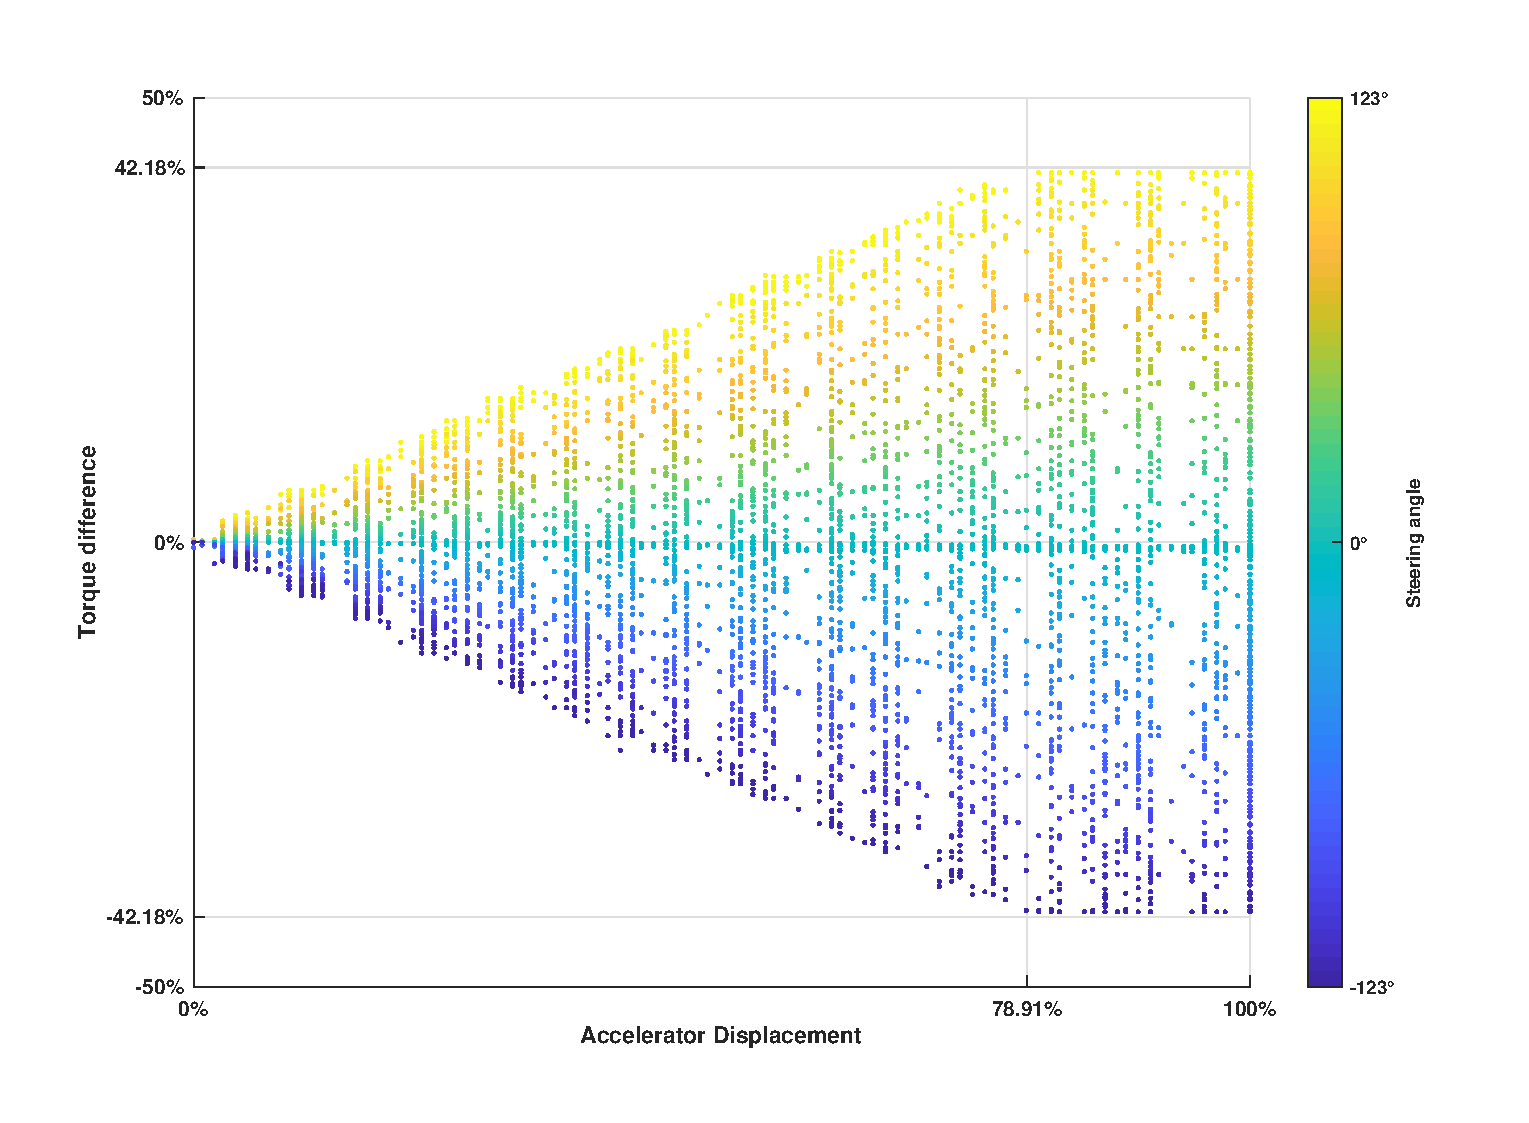
\includegraphics[width=0.46\textwidth]{figures/acc_torq.eps}
            %\caption{Measured correlation against idealised model}
            \label{diff_sum_b}
        }
        \caption{Relation between acceleration pedal displacement, steering wheel angle and normalised torque difference}
    \label{diff_sum}
\end{figure}

As one can notice in \ref{diff_sum_b} motor torque difference is linearly proportional to acceleration pedal and steering wheel displacement. This relation is clearly maintained for first $\sim80\%$ of pedal travel and it saturates on torque difference equal about $42\%$ in rest of the scale. It is the desired behaviour of this control. To explain all the values let me refer to equations \ref{diff_eq} and \ref{diff_eq_w} from the theory section.

In the vehicle, I have been working on has the maximum steering angle of 36°, wheelbase 1740mm and track equal to 1270mm. Taking these values together into mentioned equations results in wheel disproportion: 

\begin{equation*}
    \alpha_{inner} = 0.7349 ~~~~~
    \alpha_{outer} = 1.2651
\end{equation*}

From this point target torque is calculated simply by multiplication with the percent of pedal displacement and maximum torque. What is reflected in measurements for first $80\%$ of pedal travel. 
Behaviour in remaining $20\%$ is a result of limited power and accompanying safety feature described in \ref{diff_meth}. To make differential functional while using near full available power desired torque is scaled down to the maximum torque per wheel is never exceed (equation \ref{diff_saf}).
The functionality is simply active if only: \begin{equation*}
    \alpha_{outer} * d_{acc}>1
\end{equation*} 
Where:
\begin{description}
    \item[$d_{acc}$] acceleration pedal displacement
\end{description}

\begin{wrapfigure}{!r}{0.5\textwidth}
    \vspace{-20pt}
    \centering
    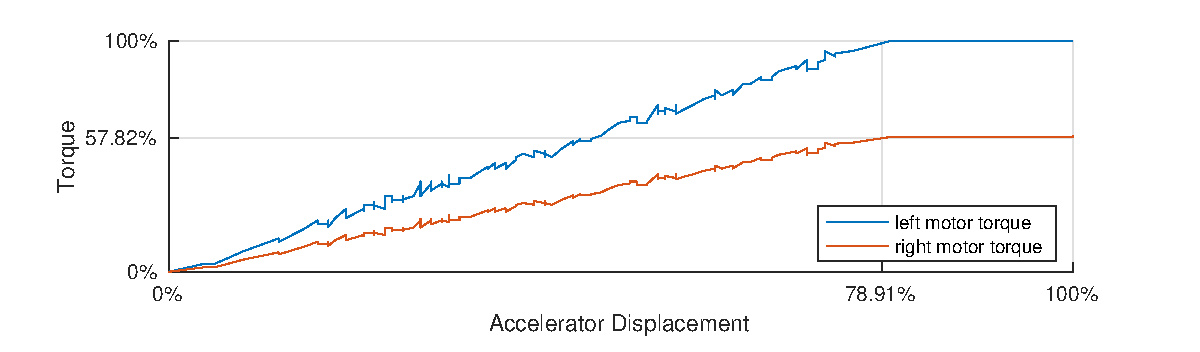
\includegraphics[width=0.46\textwidth]{figures/diff_123}
    \caption{Motors torque compassion for steering wheel rotated 124° (maximum steering angle) left}
    \label{diff_123}
    \vspace{-20pt}
\end{wrapfigure}
So taking into consideration maximum steering angle it becomes active for $d_{acc} \approx 78.91\%$ which can been seen in figure \ref{diff_sum_b}.

To further confirm this safety functionality figure \ref{diff_123} consist only of samples for maximum steering angle independently showing the torque of two wheels. The outer wheel saturates on maximum torque where the inner one maintains proportion needed for differential steering.

\section{System performance}
As mentioned due to the malfunctioning motor controller the system performance was limited. However, as I am going to show in the next figures implemented workaround performs considerably well and is not a bottleneck in a current state.

Place where the timing is the most important is in between receiving of pedal/steering wheel status and sending torque control signal to drives.
\begin{figure}[h]
    \centering
            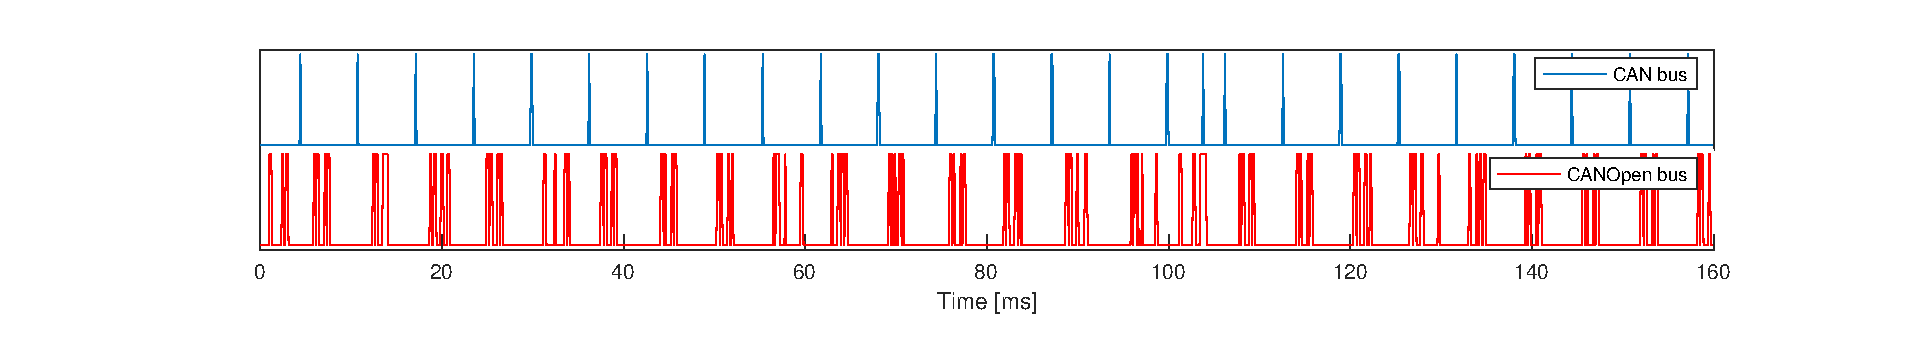
\includegraphics[width=0.8\textwidth]{figures/perf_rep.eps}
            \caption{CAN and CANOpen timing overview}
            \label{perf_over}
\end{figure}

As shown in the figure \ref{perf_over} there are messages on the CAN bus which appears within a constant interval of about $6,8 ms$. Each of these messages contains break, accelerator and steering wheel position and the timing is close to one estimated in method chapter (\ref{pedal_ideal_time}) of $5,2 ms$.

Each sensors position message is closely followed by four messages on CANOpen bus which are responsible for accordingly changing target torque values in motor controllers. 
\begin{figure}[h]
    \centering
            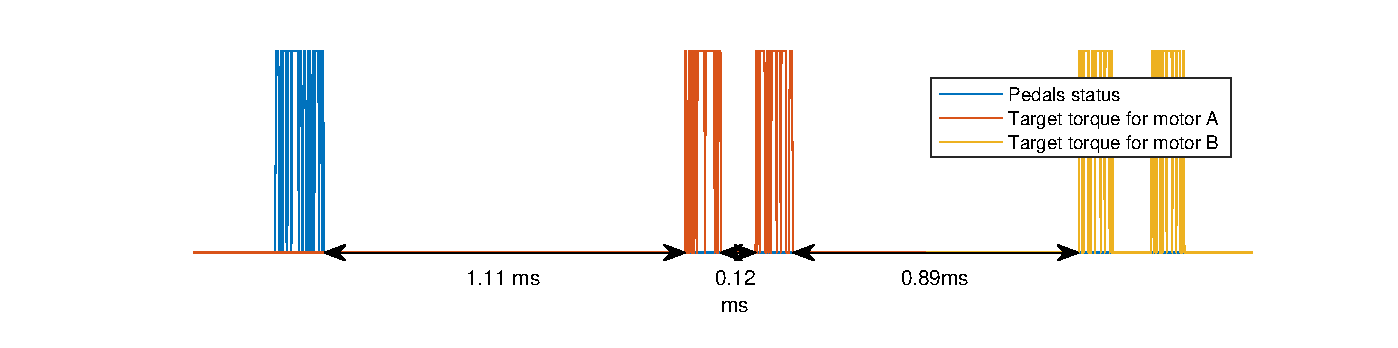
\includegraphics[width=0.8\textwidth]{figures/perf.eps}
            \caption{Control torque loop timing}
            \label{perf}
\end{figure}
As shown in figure \ref{perf} after receiving it takes just $~1.11 ms$ to first respond and second respond is sent in $~0.89 ms$ after. As in the code, two calls to LabVIEW closed library responsible for CANOpen communication are issued one after another, it suggests that in both cases about $0.89 ms$ is taken to just send a message. Therefore I am convinced that CAN receive code, interrupt issue it service and torque calculations take only about $0.22 ms$ of total time.